\documentclass[a4paper,12pt]{article}
\usepackage{amsmath}
\usepackage{amssymb}
\usepackage[polish]{babel}
\usepackage{polski}
\usepackage[utf8]{inputenc}
\usepackage{indentfirst}
\usepackage{geometry}
\usepackage{array}

\usepackage[pdftex]{color,graphicx}
\usepackage{subfigure}
\usepackage{afterpage}
\usepackage{setspace}
\usepackage{color}
\usepackage{wrapfig}
\usepackage{listings}
\usepackage{datetime}
\usepackage{hyperref}


\hypersetup{
  colorlinks   = true, %Colours links instead of ugly boxes
  urlcolor     = blue, %Colour for external hyperlinks
  linkcolor    = blue, %Colour of internal links
  citecolor   = red %Colour of citations
}


\renewcommand{\onehalfspacing}{\setstretch{1.6}}

\geometry{tmargin=2.5cm,bmargin=2.5cm,lmargin=2.5cm,rmargin=2.5cm}
\setlength{\parindent}{1cm}
\setlength{\parskip}{0mm}

\newenvironment{lista}{
\begin{itemize}
  \setlength{\itemsep}{1pt}
  \setlength{\parskip}{0pt}
  \setlength{\parsep}{0pt}
}{\end{itemize}}

\newcommand{\linia}{\rule{\linewidth}{0.4mm}}

\definecolor{lbcolor}{rgb}{0.95,0.95,0.95}
\lstset{
    backgroundcolor=\color{lbcolor},
    tabsize=4,
  language=C++,
  captionpos=b,
  tabsize=3,
  frame=lines,
  numbers=left,
  numberstyle=\tiny,
  numbersep=5pt,
  breaklines=true,
  showstringspaces=false,
  basicstyle=\footnotesize,
  identifierstyle=\color{magenta},
  keywordstyle=\color[rgb]{0,0,1},
  commentstyle=\color{Darkgreen},
  stringstyle=\color{red}
  }
\begin{document}

\noindent
\begin{tabular}{|c|p{11cm}|c|} \hline 
Grupa 1 & Kamil Sacha, Konrad Szwedo & \ddmmyyyydate\today \tabularnewline
\hline 
\end{tabular}

\renewcommand{\lstlistingname}{Listing kodu}

\section*{Zadanie 5 - Rozmycie Gaussa w OpenMPI}

Naszym zadaniem laboratoryjnym było napisanie programu wykonującego rozmycie Gaussa, w oparciu o środowisko do zrównoleglenia kodu: OpenMPI. 
Algorytm Gaussa polega na zastąpieniu pikseli obrazu wejściowego, średnią z obszaru otaczającego ten piksel. W naszym przypadku rozpatrywaliśmy maskę wielkości \(5 \times 5\), czyli do obliczenia musieliśmy znać wszystkie 25 wartości trzech kanałów rozpatrywanego piksela (kanały zapisane odpowiednio w kolejności B - Niebieski, G - Zielony, R - Czerwony). Jako wartość poszczególnego kanału (B, G, R) ustawiamy średnią z całości rozpatrywanego obszaru dla konkretnego kanału. 

\subsection*{Algorytm obliczeń}

	Głównym problemem w wykonaniu tego zadania był odpowiedni podział obrazu wejściowego tak aby każdy proces miał odpowiednią 
	porcję danych potrzebną do obliczeń. 
	Proces MASTER wykonujący główne operacje w programie jest odpowiedzialny za sprawdzenie poprawności danych wejściowych,
	 wczytanie obrazu, zapis rozmytego obrazu. 
	Jest również odpowiedzialny za przydzielenie pozostałym procesom zadań i odbiór wyników. 
	Proces główny MASTER, dzieli ilość wierszy na wszystkie obecne procesy (również dla samego siebie) i 
	wysyła je do czekających na dane procesów. Korzystamy z funkcji która zwraca podział obrazu w zależności od całkowitej ilości wierszy,
	 całkowitej ilości procesów oraz numeru procesu dla którego pytamy o wynik. 
	 Przykładowo gdy mamy 100 wierszy i uruchamiamy program dla 3 procesów wtedy procesy 
	 $P_0$= 33, $P_1$=33, $P_2$=34 otrzymują podaną ilość wierszy.
	 Ponadto zerowy proces musi otrzymać dodatkowo 2 wiersze (wiersze od 33 do 35)
	 ostatni proces także dostaje dwa wiersze poniżej (wiersze od 64 do 100),
	 natomiast procesy środkowe w naszym przykładzie $P_1$ dostają dodatkowe 4 wiersze (wiersze od 31 do 68). 
	 Nadmiarowe wiersze potrzebne są do obliczenia prawidłowej ilości wierszy wynikowych (wynikowo zawsze 4 mniej) 
	 związane jest to oczywiście z zastosowaną przez nas maską 5x5.
	 
	\begin{lstlisting}[caption=Funkcja dzieląca procesy.=Row pointery]	
int getRowsCountForProcess(int totalRows, int totalProcesses, int currentProcessCount) {

	int rows = 0;

	if (totalProcesses == 1) {
		return totalRows;
	}

	rows = totalRows / totalProcesses;

	if (currentProcessCount + 1 == totalProcesses) {
		rows += totalRows % totalProcesses;
	}

	return rows;
}		
		\end{lstlisting}

Powyższy listing kodu pokazuje początkowy algorytm podziału ilości wierszy dla procesów. 
Wszystkie procesy otrzymują po równo ilość wierszy, poza ostatnim, który otrzymuje to co zostało w puli. 
Pierwszy proces  dostaje: getRowsCountForProcess + 2 wierszy. 
Środkowe procesy dostają: getRowsCountForProcess + 4 wierszy z offsetem wierszy na -2 od bieżącego.
Ostatni  proces  dostaje: getRowsCountForProcess + 2 wierszy z offsetem wierszy na -2 od bieżącego.

\section*{Wyniki i wnioski}

     Jak możemy się spodziewać, czas wykonania programu zmniejsza się dla większej niż 1 liczbie procesów. 
     Niestety zaobserwowany wzrost przyśpieszenia nie jest liniowy. Związane jest to przede wszystkim z dużym narzutem 
     na kopiowanie danych. Dla obrazu "1.jpg" posiadającego 3 kanały każdy po 1 bajt wielkość transmisji równa będzie około 309 MiB
      (minus część nieprzesyłana, którą oblicza proces MASTER). Jest to ilość potrzebna do wysłania w jedną stronę, 
      a dane początkowe musimy jednak najpierw wysłać a potem odebrać wyniki. 
      Wartość czasu wykonania dla 5 procesów większa niż dla 4, najprawdopodobniej jest związana z obecnością 4 rdzeni fizycznych 
      reszta rdzeni jest dublowana w technologii HyperThreading, która to nie odzwierciedla wydajności jak fizyczne rdzenie. 
      Innym problemem wskazującym na dane wyniki, jest problem prawidłowego sprawdzania czasu wykonania. 
      Nie jesteśmy w stanie zmierzyć dokładnego czasu wykonań funkcji realizujących rozmycie Gauss'a, do tego czasu również wliczamy 
      jest okres poświęcony na odbiór wyników z procesów.
     


\begin{figure}
	\begin{center}
 		% GNUPLOT: LaTeX picture with Postscript
\begingroup
  \makeatletter
  \providecommand\color[2][]{%
    \GenericError{(gnuplot) \space\space\space\@spaces}{%
      Package color not loaded in conjunction with
      terminal option `colourtext'%
    }{See the gnuplot documentation for explanation.%
    }{Either use 'blacktext' in gnuplot or load the package
      color.sty in LaTeX.}%
    \renewcommand\color[2][]{}%
  }%
  \providecommand\includegraphics[2][]{%
    \GenericError{(gnuplot) \space\space\space\@spaces}{%
      Package graphicx or graphics not loaded%
    }{See the gnuplot documentation for explanation.%
    }{The gnuplot epslatex terminal needs graphicx.sty or graphics.sty.}%
    \renewcommand\includegraphics[2][]{}%
  }%
  \providecommand\rotatebox[2]{#2}%
  \@ifundefined{ifGPcolor}{%
    \newif\ifGPcolor
    \GPcolortrue
  }{}%
  \@ifundefined{ifGPblacktext}{%
    \newif\ifGPblacktext
    \GPblacktextfalse
  }{}%
  % define a \g@addto@macro without @ in the name:
  \let\gplgaddtomacro\g@addto@macro
  % define empty templates for all commands taking text:
  \gdef\gplbacktext{}%
  \gdef\gplfronttext{}%
  \makeatother
  \ifGPblacktext
    % no textcolor at all
    \def\colorrgb#1{}%
    \def\colorgray#1{}%
  \else
    % gray or color?
    \ifGPcolor
      \def\colorrgb#1{\color[rgb]{#1}}%
      \def\colorgray#1{\color[gray]{#1}}%
      \expandafter\def\csname LTw\endcsname{\color{white}}%
      \expandafter\def\csname LTb\endcsname{\color{black}}%
      \expandafter\def\csname LTa\endcsname{\color{black}}%
      \expandafter\def\csname LT0\endcsname{\color[rgb]{1,0,0}}%
      \expandafter\def\csname LT1\endcsname{\color[rgb]{0,1,0}}%
      \expandafter\def\csname LT2\endcsname{\color[rgb]{0,0,1}}%
      \expandafter\def\csname LT3\endcsname{\color[rgb]{1,0,1}}%
      \expandafter\def\csname LT4\endcsname{\color[rgb]{0,1,1}}%
      \expandafter\def\csname LT5\endcsname{\color[rgb]{1,1,0}}%
      \expandafter\def\csname LT6\endcsname{\color[rgb]{0,0,0}}%
      \expandafter\def\csname LT7\endcsname{\color[rgb]{1,0.3,0}}%
      \expandafter\def\csname LT8\endcsname{\color[rgb]{0.5,0.5,0.5}}%
    \else
      % gray
      \def\colorrgb#1{\color{black}}%
      \def\colorgray#1{\color[gray]{#1}}%
      \expandafter\def\csname LTw\endcsname{\color{white}}%
      \expandafter\def\csname LTb\endcsname{\color{black}}%
      \expandafter\def\csname LTa\endcsname{\color{black}}%
      \expandafter\def\csname LT0\endcsname{\color{black}}%
      \expandafter\def\csname LT1\endcsname{\color{black}}%
      \expandafter\def\csname LT2\endcsname{\color{black}}%
      \expandafter\def\csname LT3\endcsname{\color{black}}%
      \expandafter\def\csname LT4\endcsname{\color{black}}%
      \expandafter\def\csname LT5\endcsname{\color{black}}%
      \expandafter\def\csname LT6\endcsname{\color{black}}%
      \expandafter\def\csname LT7\endcsname{\color{black}}%
      \expandafter\def\csname LT8\endcsname{\color{black}}%
    \fi
  \fi
  \setlength{\unitlength}{0.0500bp}%
  \begin{picture}(7200.00,5040.00)%
    \gplgaddtomacro\gplbacktext{%
      \csname LTb\endcsname%
      \put(1078,704){\makebox(0,0)[r]{\strut{} 1000}}%
      \csname LTb\endcsname%
      \put(1078,1111){\makebox(0,0)[r]{\strut{} 1500}}%
      \csname LTb\endcsname%
      \put(1078,1518){\makebox(0,0)[r]{\strut{} 2000}}%
      \csname LTb\endcsname%
      \put(1078,1925){\makebox(0,0)[r]{\strut{} 2500}}%
      \csname LTb\endcsname%
      \put(1078,2332){\makebox(0,0)[r]{\strut{} 3000}}%
      \csname LTb\endcsname%
      \put(1078,2740){\makebox(0,0)[r]{\strut{} 3500}}%
      \csname LTb\endcsname%
      \put(1078,3147){\makebox(0,0)[r]{\strut{} 4000}}%
      \csname LTb\endcsname%
      \put(1078,3554){\makebox(0,0)[r]{\strut{} 4500}}%
      \csname LTb\endcsname%
      \put(1078,3961){\makebox(0,0)[r]{\strut{} 5000}}%
      \csname LTb\endcsname%
      \put(1078,4368){\makebox(0,0)[r]{\strut{} 5500}}%
      \csname LTb\endcsname%
      \put(1078,4775){\makebox(0,0)[r]{\strut{} 6000}}%
      \csname LTb\endcsname%
      \put(1210,484){\makebox(0,0){\strut{} 0}}%
      \csname LTb\endcsname%
      \put(1909,484){\makebox(0,0){\strut{} 2}}%
      \csname LTb\endcsname%
      \put(2608,484){\makebox(0,0){\strut{} 4}}%
      \csname LTb\endcsname%
      \put(3307,484){\makebox(0,0){\strut{} 6}}%
      \csname LTb\endcsname%
      \put(4007,484){\makebox(0,0){\strut{} 8}}%
      \csname LTb\endcsname%
      \put(4706,484){\makebox(0,0){\strut{} 10}}%
      \csname LTb\endcsname%
      \put(5405,484){\makebox(0,0){\strut{} 12}}%
      \csname LTb\endcsname%
      \put(6104,484){\makebox(0,0){\strut{} 14}}%
      \csname LTb\endcsname%
      \put(6803,484){\makebox(0,0){\strut{} 16}}%
      \put(176,2739){\rotatebox{-270}{\makebox(0,0){\strut{}Średni czas wykonania [ms]}}}%
      \put(4006,154){\makebox(0,0){\strut{}Ilość wątków}}%
    }%
    \gplgaddtomacro\gplfronttext{%
      \csname LTb\endcsname%
      \put(5816,4602){\makebox(0,0)[r]{\strut{}Czas wykonania}}%
    }%
    \gplbacktext
    \put(0,0){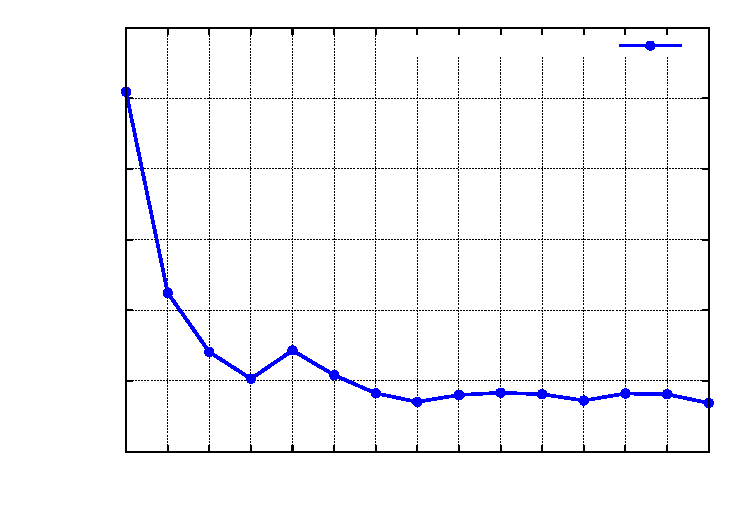
\includegraphics{wykres_czasu}}%
    \gplfronttext
  \end{picture}%
\endgroup

	\end{center}
	
    \caption{Wykres zależności czasu wykonania od ilości procesów.
     Dla obrazu wejściowego '1.jpg' o wymiarach \(24107 \times 4491 \approx 10^9\) pikseli.}

\end{figure}



\begin{figure}
	\begin{center}
 		% GNUPLOT: LaTeX picture with Postscript
\begingroup
  \makeatletter
  \providecommand\color[2][]{%
    \GenericError{(gnuplot) \space\space\space\@spaces}{%
      Package color not loaded in conjunction with
      terminal option `colourtext'%
    }{See the gnuplot documentation for explanation.%
    }{Either use 'blacktext' in gnuplot or load the package
      color.sty in LaTeX.}%
    \renewcommand\color[2][]{}%
  }%
  \providecommand\includegraphics[2][]{%
    \GenericError{(gnuplot) \space\space\space\@spaces}{%
      Package graphicx or graphics not loaded%
    }{See the gnuplot documentation for explanation.%
    }{The gnuplot epslatex terminal needs graphicx.sty or graphics.sty.}%
    \renewcommand\includegraphics[2][]{}%
  }%
  \providecommand\rotatebox[2]{#2}%
  \@ifundefined{ifGPcolor}{%
    \newif\ifGPcolor
    \GPcolortrue
  }{}%
  \@ifundefined{ifGPblacktext}{%
    \newif\ifGPblacktext
    \GPblacktextfalse
  }{}%
  % define a \g@addto@macro without @ in the name:
  \let\gplgaddtomacro\g@addto@macro
  % define empty templates for all commands taking text:
  \gdef\gplbacktext{}%
  \gdef\gplfronttext{}%
  \makeatother
  \ifGPblacktext
    % no textcolor at all
    \def\colorrgb#1{}%
    \def\colorgray#1{}%
  \else
    % gray or color?
    \ifGPcolor
      \def\colorrgb#1{\color[rgb]{#1}}%
      \def\colorgray#1{\color[gray]{#1}}%
      \expandafter\def\csname LTw\endcsname{\color{white}}%
      \expandafter\def\csname LTb\endcsname{\color{black}}%
      \expandafter\def\csname LTa\endcsname{\color{black}}%
      \expandafter\def\csname LT0\endcsname{\color[rgb]{1,0,0}}%
      \expandafter\def\csname LT1\endcsname{\color[rgb]{0,1,0}}%
      \expandafter\def\csname LT2\endcsname{\color[rgb]{0,0,1}}%
      \expandafter\def\csname LT3\endcsname{\color[rgb]{1,0,1}}%
      \expandafter\def\csname LT4\endcsname{\color[rgb]{0,1,1}}%
      \expandafter\def\csname LT5\endcsname{\color[rgb]{1,1,0}}%
      \expandafter\def\csname LT6\endcsname{\color[rgb]{0,0,0}}%
      \expandafter\def\csname LT7\endcsname{\color[rgb]{1,0.3,0}}%
      \expandafter\def\csname LT8\endcsname{\color[rgb]{0.5,0.5,0.5}}%
    \else
      % gray
      \def\colorrgb#1{\color{black}}%
      \def\colorgray#1{\color[gray]{#1}}%
      \expandafter\def\csname LTw\endcsname{\color{white}}%
      \expandafter\def\csname LTb\endcsname{\color{black}}%
      \expandafter\def\csname LTa\endcsname{\color{black}}%
      \expandafter\def\csname LT0\endcsname{\color{black}}%
      \expandafter\def\csname LT1\endcsname{\color{black}}%
      \expandafter\def\csname LT2\endcsname{\color{black}}%
      \expandafter\def\csname LT3\endcsname{\color{black}}%
      \expandafter\def\csname LT4\endcsname{\color{black}}%
      \expandafter\def\csname LT5\endcsname{\color{black}}%
      \expandafter\def\csname LT6\endcsname{\color{black}}%
      \expandafter\def\csname LT7\endcsname{\color{black}}%
      \expandafter\def\csname LT8\endcsname{\color{black}}%
    \fi
  \fi
  \setlength{\unitlength}{0.0500bp}%
  \begin{picture}(7200.00,5040.00)%
    \gplgaddtomacro\gplbacktext{%
      \csname LTb\endcsname%
      \put(682,704){\makebox(0,0)[r]{\strut{} 0}}%
      \csname LTb\endcsname%
      \put(682,1722){\makebox(0,0)[r]{\strut{} 1}}%
      \csname LTb\endcsname%
      \put(682,2740){\makebox(0,0)[r]{\strut{} 2}}%
      \csname LTb\endcsname%
      \put(682,3757){\makebox(0,0)[r]{\strut{} 3}}%
      \csname LTb\endcsname%
      \put(682,4775){\makebox(0,0)[r]{\strut{} 4}}%
      \csname LTb\endcsname%
      \put(814,484){\makebox(0,0){\strut{} 1}}%
      \csname LTb\endcsname%
      \put(1242,484){\makebox(0,0){\strut{} 2}}%
      \csname LTb\endcsname%
      \put(1670,484){\makebox(0,0){\strut{} 3}}%
      \csname LTb\endcsname%
      \put(2097,484){\makebox(0,0){\strut{} 4}}%
      \csname LTb\endcsname%
      \put(2525,484){\makebox(0,0){\strut{} 5}}%
      \csname LTb\endcsname%
      \put(2953,484){\makebox(0,0){\strut{} 6}}%
      \csname LTb\endcsname%
      \put(3381,484){\makebox(0,0){\strut{} 7}}%
      \csname LTb\endcsname%
      \put(3809,484){\makebox(0,0){\strut{} 8}}%
      \csname LTb\endcsname%
      \put(4236,484){\makebox(0,0){\strut{} 9}}%
      \csname LTb\endcsname%
      \put(4664,484){\makebox(0,0){\strut{} 10}}%
      \csname LTb\endcsname%
      \put(5092,484){\makebox(0,0){\strut{} 11}}%
      \csname LTb\endcsname%
      \put(5520,484){\makebox(0,0){\strut{} 12}}%
      \csname LTb\endcsname%
      \put(5947,484){\makebox(0,0){\strut{} 13}}%
      \csname LTb\endcsname%
      \put(6375,484){\makebox(0,0){\strut{} 14}}%
      \csname LTb\endcsname%
      \put(6803,484){\makebox(0,0){\strut{} 15}}%
      \put(176,2739){\rotatebox{-270}{\makebox(0,0){\strut{}Średnie przyśpieszenie}}}%
      \put(3808,154){\makebox(0,0){\strut{}Liczba wątków}}%
    }%
    \gplgaddtomacro\gplfronttext{%
      \csname LTb\endcsname%
      \put(5816,877){\makebox(0,0)[r]{\strut{}Przyśpieszenie}}%
    }%
    \gplbacktext
    \put(0,0){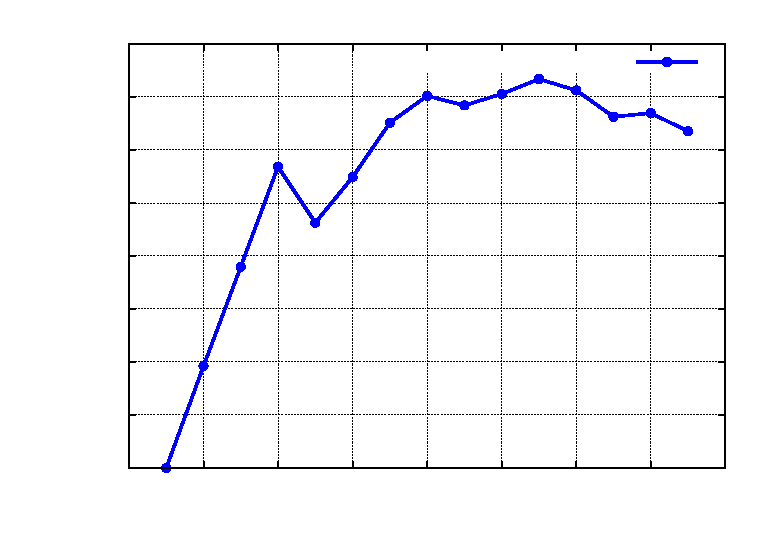
\includegraphics{dane/wykres_przyspieszenia}}%
    \gplfronttext
  \end{picture}%
\endgroup
   		 		
	\end{center}
	
    \caption{Wykres zależności przyśpieszenia od ilości procesów.
     Dla obrazu wejściowego '1.jpg' o wymiarach \(24107 \times 4491 \approx 10^9\) pikseli.}
\end{figure}

\end{document}
